\chapter{Introduction} \label{chap:intro}

Video Quality Assessment (VQA) is a pivotal domain in visual communication systems and computer vision, which enable accurate evaluation of perceived video quality to optimize user experience and enhance image processing workflows. Recent analyses indicate that video accounts for almost two thirds of global internet traffic~\cite{sandvine_global_2023}, underscoring the importance of robust VQA methods. These methods are integral to applications involving image acquisition, compression, transmission, and display, especially as digital media continue to dominate both professional and consumer contexts. High-performance VQA techniques assess the fidelity and quality degradation introduced throughout the media pipeline, effectively identifying artifacts such as blurring, blocking, noise, and other distortions that compromise visual integrity.

\section{A Video Quality Assessment Perspective} \label{sec:se1}

Modern applications increasingly depend on reliable metrics to evaluate the quality of the media, ensuring compatibility with the complex demands of media pipelines and the intricacies of the human visual system (HVS). As digital media consumption grows, there is a critical need for well-defined tools that can effectively assess the quality of transmitted content. To address this need, video quality assessment methodologies are broadly categorized into two classes: subjective and objective. 

Subjective assessment, such as the double stimulation methods of the standardized mean opinion score (MOS) defined in the ITU recommendations \cite{itu2017p800}, is based on human evaluators to gauge perceived quality. The Mean Opinion Score (MOS) represents the definitive subjective metric for media quality assessment. This psychometric scale quantifies perceived quality through human evaluations, employing a five-point Likert-type scale. MOS serves as the gold standard for subjective testing across telecommunications and multimedia systems, providing empirically validated ground truth for perceptual quality evaluation. The methodology requires controlled laboratory conditions, standardized test stimuli, and statistically significant participant cohorts (typically $n \geq 15$) to ensure reliability, as specified in ITU-T P.800's \cite{itu2017p800} rigorous experimental protocols.  
Objective assessment, on the other hand, employs computational metrics and is further divided into three established approaches: Full reference (FR), reduced reference (RR) and no reference (NR). FR methods compare the degraded content with a pristine reference, making them highly effective in controlled environments where reference data is available. RR methods rely on partial access to reference features, offering a balance between accuracy and adaptability in constrained scenarios. NR methods, on the other hand, operate without any reference and are indispensable for real-time applications, such as live streaming, where reference data can be unavailable or impractical. The development of NR methods is particularly challenging but essential for dynamic systems that require instantaneous quality assessment. 

Traditional VQA approaches predominantly follow a knowledge-based paradigm, in which hand-crafted features are extracted manually to evaluate video quality. Examples include extensions of NR Image Quality Assessment (IQA) methods, such as NIQE~\cite{mittal2012no}, IL-NIQE~\cite{zhang2015feature}, and BRISQUE~\cite{mittal2012completely}, adapted to the video domain. These methods rely heavily on predefined quality indicators to perform evaluations, limiting their scalability in complex scenarios. 

In contrast, data-driven NR VQA models leverage the power of neural networks to automatically extract quality-aware features from distorted videos, offering a simpler yet more robust alternative. These models can be classified into three categories based on their training methodologies: those using pre-trained models, end-to-end training frameworks, and unsupervised learning approaches. By dynamically learning quality features, data-driven approaches demonstrate superior adaptability and performance, especially in diverse and unpredictable environments.

Subjective assessment, considered the most reliable, depends on human visual perception and aims to replicate the qualitative judgment of a human observer. However, subjective assessments are inherently time-consuming, costly, and impractical for real-time applications, where immediate feedback is necessary. To address these limitations, objective VQA methods have been widely adopted. These algorithms can be designed to predict subjective quality automatically, allowing for efficient and scalable assessment suitable for automated systems.

\subsection{Challenges and Opportunities in Advanced Video Quality Assessment}

Despite significant advancements in Video Quality Assessment (VQA) methodologies, contemporary approaches encounter substantial limitations when evaluating real-time, no-reference video quality with high precision, particularly in dynamic contexts such as live streaming and automated quality monitoring systems. Traditional Full-Reference (FR) and Reduced-Reference (RR) methodologies demonstrate inherent inadequacies in scenarios where reference data remains inaccessible, while No-Reference (NR) VQA frameworks, despite their theoretical promise, frequently struggle to achieve an optimal equilibrium between computational efficiency and perceptual accuracy. As elucidated in a comprehensive contemporary survey by Min et al.~\cite{min2024perceptual}, the majority of NR methodologies are constrained by their dependence on manually engineered features or conventional machine learning paradigms, which frequently fail to encapsulate the multifaceted perceptual qualities that align with the sophisticated mechanisms of the human visual system (HVS).

In response to these challenges, this dissertation investigates not only the machine learning methodology itself but also the programming environment in which such methodologies are deployed. The model is implemented, trained and tested in a Python environment and its inference on a real-time streaming scenario run using the Rust, a programming language that has gained prominence due to its unique balance between performance, safety, and concurrency.

The decision to use Rust is motivated by both academic and industrial findings. According to Fulton et al.~\cite{fulton2022benefits}, Rust offers notable advantages including high-quality tooling, comprehensive documentation, lifecycle benefits for development, and a positive influence on secure coding practices. These characteristics make Rust particularly attractive for building reliable real-time systems such as media pipelines for VQA inference.

Furthermore, an industrial case study by Johansson and Rappe~\cite{johansson2023transitioning} evaluating the transition from C to Rust in media streaming development found that although Rust incurs a modest performance penalty—approximately 4.24\% longer execution time compared to C—the trade-off is justified by gains in safety, maintainability, and long-term reliability. These results underscore Rust’s practical viability in performance-sensitive domains and support its adoption in the deployment of machine learning models within high-throughput audiovisual environments.

Thus, the use of Rust in this dissertation is not incidental but central to the research theme, exploring how its language design and ecosystem can support the operationalization of advanced, attention-based QoE prediction models in streaming applications.

\subsection{Cross-Sectoral Implications of Advanced No-Reference VQA Systems}

The successful conceptualization and implementation of a robust, artificial intelligence-driven NR VQA framework presents profound implications across diverse industrial sectors that rely on high-fidelity visual content transmission and analysis. Within the domain of digital media distribution, such an advanced model can substantially enhance streaming service quality through the provision of instantaneous feedback regarding image fidelity, consequently elevating viewer experience metrics and augmenting customer retention rates. Similarly, telecommunications applications, particularly video conferencing platforms and virtual reality environments, stand to benefit considerably from such technological innovations, as maintaining optimal video quality constitutes a fundamental prerequisite for preserving immersive experiences and facilitating effective interpersonal communication. Furthermore, in the increasingly significant domain of autonomous systems, including aerial drones and robotic vision applications, a sophisticated NR VQA model can substantially enhance decision-making processes by enabling these systems to evaluate and dynamically adapt to fluctuating visual conditions without computational latency. Additionally, the strategic integration of this technology within automated quality monitoring infrastructures can optimize content delivery pipelines, simultaneously reducing manual supervisory requirements and operational expenditures while maintaining consistent quality standards.

These cross-sectoral implications are made significantly more viable and sustainable through the use of the Rust programming language as the implementation platform. Rust's unique combination of memory safety, concurrency safety, immutability by default, and absence of null pointer dereferencing contributes to building resilient systems that are critical for mission-critical, high-availability environments~\cite{fulton2022benefits}. In particular, Rust's ownership and lifetime semantics ensure deterministic behavior and prevent common bugs associated with memory corruption and data races—issues that are especially detrimental in systems handling real-time audiovisual data. Moreover, Rust's appeal also stems from its high-performance characteristics and the absence of a garbage collector, enabling developers to build low-latency systems with predictable runtime behavior. As reported by developers surveyed in Fulton et al.’s study, Rust offers a “trifecta of performance, productivity, and safety,” making it an ideal choice for deploying machine learning models in streaming media contexts where both speed and correctness are paramount~\cite{fulton2022benefits}.

In addition to real-time media systems, Rust has also demonstrated promising capabilities in embedded machine learning, particularly for resource-constrained environments. One notable example is the \emph{MicroFlow} inference engine, a lightweight and efficient Rust-based runtime for TinyML deployments~\cite{carnelos2025microflow}. Designed specifically for embedded devices in IoT applications, MicroFlow achieves highly efficient inference with neural networks while preserving Rust’s guarantees of memory safety and deterministic performance. This exemplifies Rust’s adaptability not only to high-throughput server-class workloads but also to edge computing scenarios in robotics, industrial control, and autonomous visual systems. The capacity to target both high-end and low-power hardware ecosystems further enhances the cross-sectoral deployability of NR VQA systems implemented in Rust.

\subsection{Research Contributions and Broader Impact}

By systematically addressing the multifaceted challenge of accurately assessing video quality without reference images in real-time streaming environments---particularly those incorporating actual transmission footage that has been captured and subsequently processed---where precise orchestration of VQA model inputs and outputs is paramount, this research transcends mere incremental improvement to make substantial contributions to both the computer vision and systems engineering domains. The proposed implementation acknowledges the critical importance of efficient data management within the assessment pipeline, particularly when processing authentic transmission streams rather than synthetic or laboratory-generated content.

Beyond its contributions to perceptual quality estimation and the application of advanced no-reference models such as DSA-QoE, this work introduces a novel systems-level perspective by embedding the model into an operational Rust-based media pipeline. The decision to adopt Rust, a systems programming language known for its performance, memory safety, and concurrency guarantees, constitutes a major practical contribution. It demonstrates that sophisticated machine learning inference can be deployed in real-time, safety-critical environments without relying on traditional high-overhead stacks like Python or C++ with garbage collection.

The use of Rust reinforces the overall system’s robustness and maintainability, and directly addresses long-standing challenges in safe low-level deployment of AI workloads. As demonstrated in empirical and industry-facing studies~\cite{fulton2022benefits}, Rust’s features such as memory and concurrency safety, immutability by default, and absence of null pointer dereferencing significantly reduce the surface for runtime errors---a critical factor when real-time QoE metrics must be delivered without interruption. Furthermore, Rust’s growing ecosystem for AI and embedded applications, as exemplified by platforms such as MicroFlow for TinyML inference~\cite{carnelos2025microflow}, underscores its potential as a future-proof language for cross-domain deployment of machine learning systems.

This research thus delivers not only algorithmic and architectural innovation but also a demonstration of how advanced AI models can be integrated into production-grade pipelines with systems-level engineering rigor. By doing so, it fosters technological innovation while enhancing both objective quality metrics and subjective perceptual experience of real-time audiovisual communications. It validates the operational feasibility and reliability of deploying deep learning–based VQA mechanisms in heterogeneous environments as media broadcast centers, bridging the gap between theoretical AI models and their robust, scalable application in industry.

\subsection{State-of-the-Art No-Reference Video Quality Assessment Models}

Based on recent research, the algorithms FastVQA \cite{wu2022fastvqa}, MDVSFA \cite{li2023unified}, Dual-Stage Attention \cite{jia2024continuous} and DA-QoE \cite{li2022weakly} have emerged as highly effective options for No-Reference Video Quality Assessment (NR VQA). A recent survey \cite{min2024perceptual} demonstrates their superior performance across benchmark datasets such as KoNViD-1k \cite{hosu2017konvid}, LIVE-VQC \cite{sinno2018large}, and YouTube-UGC \cite{wang2019youtube}, showcasing their ability to balance computational efficiency with perceptual accuracy. FastVQA achieves state-of-the-art results with end-to-end optimization, excelling in both speed and accuracy, as evidenced by its consistently high PLCC and SRCC scores \cite{wu2022fastvqa}. MDVSFA, on the other hand, leverages a robust pre-trained ResNet-50 backbone for feature extraction, delivering reliable and scalable results across diverse datasets \cite{li2023unified}. A performance comparison of FastVQA and MDVSFA can be assessed in Table \ref{tab:fastvqa_mdvsfa_comparison}

\begin{figure}
    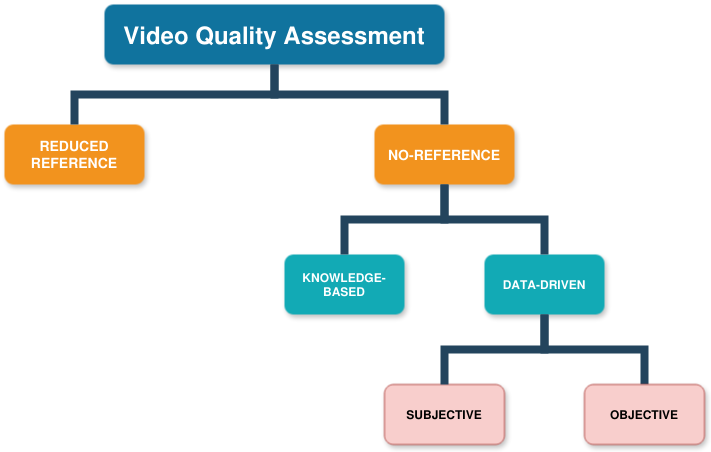
\includegraphics[width=0.86\textwidth]{figures/vqa_diagram.png}
    \caption{Visual Quality Assessment diagram}
    \label{fig:arch}
\end{figure}

\begin{table}[ht]
\centering
\caption{Performance comparison of FastVQA and MDVSFA on different databases. Spearman's Rank Correlation Coefficient (SRCC) and Pearson Linear Correlation Coefficient (PLCC).}
\label{tab:fastvqa_mdvsfa_comparison}
\begin{tabular}{lccc}
\hline
\textbf{Algorithm} & \textbf{Dataset} & \textbf{SRCC} & \textbf{PLCC} \\
\hline
FastVQA & KoNViD-1k    & 0.891 & 0.892 \\
FastVQA & LIVE-VQC     & 0.865 & 0.865 \\
FastVQA & YouTube-UGC  & 0.855 & 0.852 \\
\hline
MDVSFA  & KoNViD-1k    & 0.781 & 0.785 \\
MDVSFA  & LIVE-VQC     & 0.773 & 0.780 \\
MDVSFA  & YouTube-UGC  & 0.749 & 0.746 \\
\hline
\end{tabular}
\end{table}

The Dual-Stage Attention approach introduces a novel architecture that processes video quality assessment in two distinct attention-driven stages \cite{jia2024continuous}. In the first stage, it focuses on spatial features within frames, while the second stage emphasizes temporal relationships across sequential frames, allowing it to capture both spatial distortions and temporal inconsistencies that affect perceived quality. As shown in Table~\ref{tab:dsa_performance}, the Dual-Stage Attention model achieves impressive performance across multiple datasets, particularly when utilizing combined MSE and PLCC loss functions. Meanwhile, DA-QoE (Domain-Adaptive Quality of Experience) employs a weakly supervised learning framework that addresses the domain gap between different datasets, enabling more generalizable quality predictions across diverse video content \cite{li2022weakly}. This is particularly valuable when training data may not fully represent real-world conditions. Table~\ref{tab:da_qoe_performance} further illustrates DA-QoE's strong correlation with human perceptual judgments.

\begin{table}[ht]
\centering
\caption{Performance of Dual-Stage Attention model on different databases. Spearman's Rank Correlation Coefficient (SRCC) and Pearson Linear Correlation Coefficient (PLCC).}
\label{tab:dsa_performance}
\begin{tabular}{lccc}
\hline
\textbf{Dataset} & \textbf{SRCC} & \textbf{PLCC} \\
\hline
Waterloo-IV & 0.795 & 0.801 \\
Waterloo-III & 0.851 & 0.870 \\
LIVE-NFLX-II  & 0.915 & 0.922 \\
\hline
\end{tabular}
\end{table}

\begin{table}[ht]
\centering
\caption{Performance of DA-QoE model on different databases. Spearman's Rank Correlation Coefficient (SRCC) and Pearson Linear Correlation Coefficient (PLCC).}
\label{tab:da_qoe_performance}
\begin{tabular}{lccc}
\hline
\textbf{Dataset} & \textbf{SRCC} & \textbf{PLCC} \\
\hline
LIVE-Mobile-II & 0.7890 & 0.7985 \\
Waterloo SQoE-II & 0.8963 & 0.9156 \\
LIVE Netflix  & 0.8280 & 0.8144 \\
\hline
\end{tabular}
\end{table}

These characteristics make all four algorithms well-suited for the proposed framework, which aims to address real-time quality assessment requirements. The position of these algorithms, alongside other VQA methodologies, is illustrated in the broader context of VQA branches and approaches in Figure~\ref{fig:arch}.

\section{Dissertation Structure} \label{sec:struct}

The structure of this document is organized into five comprehensive chapters. Chapter~\ref{chap:ch2} provides a thorough \textit{Background and Literature Review on State-of-the-Art Video Quality Assessment Algorithms}, exploring key concepts and foundational prior research in the field, offering an in-depth analysis of current methodologies and their applications. Chapter~\ref{chap:ch3} presents the \textit{Preliminary Work and Workplan}, detailing a strategic roadmap for future efforts in this research. Finally, Chapter~\ref{chap:ch4} concludes the document with a summary, highlighting the implications of the work and suggesting directions for further exploration.

